% !TEX root = main.tex

Trilinos is a community-driven open-source C++ software framework and collection of reusable scientific libraries designed to enable the development of scalable, high-performance algorithms for solving complex, multiscale, and multiphysics engineering and scientific problems on advanced computing architectures.
While Trilinos can run on a variety of hardware platforms ranging from small workstations to large supercomputers, the typical use of Trilinos is on leadership-class systems with new or emerging hardware architectures.

% History
Trilinos was originally conceived as a framework of three packages for distributed memory systems. The original Trilinos publication~\cite{Heroux2005a} described the motivation, philosophy, and capabilities of Trilinos at that time. Seven years later, a two-part collection of 16 papers provided a new overview of Trilinos and many of its packages~\cite{Heroux2012,HerouxIntro2012part1,HerouxIntro2012part2,pawlowski2012automating,Oldfield2012,bochev2012,Boman2012,Baker2012,Kokkos2012,pawlowski2012automatingpart2,Spotz2012,Long2012,Morris2012,Howle2012,Bavier2012a,Gaidamour2012} and described the intervening expansion of Trilinos' capabilities and strategic goals for Trilinos. Trilinos today hews to the overall vision from two decades ago, but has evolved alongside changes in programming models, application needs, hardware architectures, and algorithms. Trilinos has grown from a library of three packages to more than fifty packages with functionality and features supporting a wide range of applications.

For much of its history, packages have relied heavily on the linear algebra classes provided by Epetra.
Epetra does not support larger problems (2B+ unknowns), nor does it allow for accelerator offload.
Since the packages of the old Epetra stack are scheduled to be archived and removed from the main Trilinos repository on GitHub by the end of 2025, this paper describes only the modern Trilinos software stack, which builds upon Tpetra and the Kokkos ecosystem to achieve performance portability across hardware architectures.

% Purpose
This article attempts to capture a snapshot the current state of Trilinos, as an update to the articles published thirteen and twenty years ago.
Therefore it focuses on the major developments within Trilinos in the last decade as well as new features and functionality that have been added to advance scientific and engineering applications.
It will give only an overview of the features, and we refer to the extensive list of references for the details of these features.
We are also cognizant of the fact that this article describes software that is being actively developed and constantly evolving.
Hence, we will focus on the high-level features and concepts that we expect to remain stable for several years.
We also briefly touch upon the Trilinos community 
%(Section~\ref{sec:community}) 
and software engineering issues with respect to Trilinos.

\subsection{Modern Trilinos:  Performance Portability through Kokkos}


A key goal of modern Trilinos is to offer a performance\hyp{}portable collection of reusable scientific libraries, allowing users to develop applications that achieve high efficiency across all modern high performance computing (HPC) hardware architectures.
This goal emerged when the HPC architecture landscape started diversifying with the
introduction of GPU acceleration for scientific software. Today, nine of the top ten systems in the Top500\footnote{https://top500.org} use GPUs, with only a single system using CPUs only. A challenge in this shift is the diversification of vendor-provided programming models: the aforementioned systems have four different preferred programming models: CUDA, HIP and SYCL for the GPU-based systems and OpenMP for the CPU system.

To avoid the necessity of diverging code paths, Trilinos leverages the Kokkos ecosystem\footnote{\url{https://kokkos.org}}~\cite{trott2021kokkos} to write performance portable code. The Kokkos ecosystem originated from the native Trilinos packages Kokkos~\cite{heroux2011toward} and Kokkos Kernels but split off a decade ago into a standalone project hosted and developed independently of Trilinos\footnote{https://github.com/kokkos}.
Now, Trilinos provides snapshots of the two primary Kokkos subprojects (Core and Kernels) that reflect the latest release of Kokkos. Trilinos can also be built against version-compatible external installations of Kokkos --- a capability required for interoperability with other Kokkos-based libraries.

Kokkos enables Trilinos developers to write single source implementations of their packages that perform well on all major HPC hardware architectures. Some of its design principles are also reflected in Trilinos API designs. In particular, the
use of \texttt{execution} and \texttt{memory spaces} as parameters of data structures and algorithms is a common thread throughout Trilinos. This design characteristic enables Trilinos users to manage the heterogeneity of modern architectures and its impact on Trilinos data structures.


\subsection{Trilinos Functionality}

%Product and package structure
%MMW I really don't see the point of emphasizing products.  We don't really give much explanation of what it means to be a Trilinos product.  I suggest we either explain products better (much better explanation of what this means) or deemphasize them.  I am going to deemphasize them for now.

The features and capabilities of Trilinos are divided into several software units called \textit{packages}.
Each Trilinos package has a well-defined set of unique capabilities that is important for scientific or engineering applications. Packages are semi-autonomous, often having their own development team, users, and set of requirements and development principles.  However, packages also follow a general set of Trilinos expectations such as having a designated point-of-contact and following software quality expectations (e.g., sufficient documentation, continuous integration testing, clearly defined dependencies, and using the Trilinos infrastructure for building and installation).

While most packages are developed natively in the Trilinos repository, some packages are developed externally and snapshotted into Trilinos.
These are (in alphabetical order):
Compadre\footnote{\url{https://github.com/sandialabs/compadre}},
Kokkos and Kokkos Kernels,
Krino,
SEACAS\footnote{\url{https://github.com/sandialabs/seacas}},
Sierra ToolKit (STK),
and TriBITS\footnote{\url{https://github.com/TriBITSPub/TriBITS}}.
Some reasons for snapshotting external packages into Trilinos include:
external packages and repositories facilitate easy and independent usage by other software projects without having to pull in Trilinos;
snapshotting provides an integration process for external packages into Trilinos, ensuring continual compatibility between all packages;
and snapshotting allows easy integration into Trilinos-based application codes, alleviating users from managing these dependencies themselves.
We refer to the Trilinos website (\url{https://trilinos.github.io}) for a brief description of these packages.

In the following sections of this paper, we group the Trilinos packages that share common objectives (e.g., solving linear systems) together into Trilinos' five \textit{product areas}:  Core, Linear Solvers and Preconditioners, Nonlinear Solvers and Analysis Tools, Discretization Tools, and Framework Infrastructure.
Trilinos' packages and their assignment to a product area are illustrated in Figure~\ref{fig:GraphicalOverview}.
\begin{figure}
\centering
% !TEX root = main.tex

% Core: Kokkos, Kokkos Kernels, Teuchos, Tpetra, Thyra (5)
% Linear Solvers and Preconditioners: Belos, Ifpack2, FROSch, MueLu, ShyLu and Amesos2, Teko, Anasazi, Stratimikos (8)
% Nonlinear Solvers and Analysis Tools: NOX & LOCA, ROL, Sacado, Stokhos, Piro (5)
% Discretizations: Intrepid2, Phalanx, Tempus, Panzer, Comparde (5)
% Framework: Build and Test Infrastructure, Documentation Infrastructure, PyTrilinos2 (3)

\begin{tikzpicture}

\definecolor{colTum}{rgb}{0.0,0.396,0.741} % TUM blue
\definecolor{colUniBwOr}{rgb}{0.929,0.431,0.0} % Unibw Orange
\definecolor{colUniBwGr}{RGB}{113,112,114} % Unibw Gray
\definecolor{myDarkGreen}{rgb}{0,0.6,0}
\definecolor{myPurple}{RGB}{125,0,255}
\definecolor{myDarkRed}{RGB}{210,0,0}
\definecolor{myYellow}{RGB}{255,202,5}
\definecolor{myPetrol}{RGB}{0,172,164}

\def\ri{4}
\def\rm{4.5}
\def\ro{5}
\def\areah{0.75}
\def\packagew{3.0}
\def\packageh{0.6}
\def\dist{0.1}
\def\colCore{myDarkRed}
\def\colNonlinear{myPetrol}
\def\colDisc{myDarkGreen}
\def\colLinear{colTum}
\def\colFrame{colUniBwOr}

\node at (0,0) {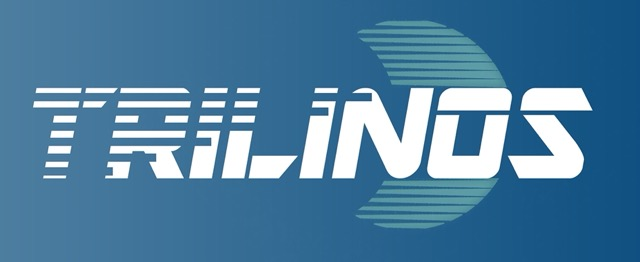
\includegraphics[width=4cm]{logo_trilinos.jpeg}};

\fill[even odd rule,gray!10] circle (\ri) circle (\ro);

\begin{scope}[shift={(84:\rm-0.3)}]
\begin{scope}[shift={(-0.5*\packagew,-2.5*\packageh)}]
% Core: Kokkos, Kokkos Kernels, Teuchos, Tpetra, Thyra (5)
\draw [fill=\colCore!20] (-\dist-\areah,-\dist) rectangle (\packagew+\dist, 5*\packageh+5*\dist);
\node [rotate=90,align=center] at (-0.5*\dist-0.5*\areah,2*\dist+2.5*\packageh) {\textbf{Core}};
\draw [fill=\colCore!40] (0,0) rectangle (\packagew, \packageh) node [pos=0.5] {Thyra};
\draw [fill=\colCore!40] (0,\packageh+1*\dist) rectangle (\packagew, 2*\packageh+1*\dist) node [pos=0.5] {Tpetra};
\draw [fill=\colCore!40] (0,2*\packageh+2*\dist) rectangle (\packagew, 3*\packageh+2*\dist) node [pos=0.5] {Teuchos};
\draw [fill=\colCore!40,dashed] (0,3*\packageh+3*\dist) rectangle (\packagew, 4*\packageh+3*\dist) node [pos=0.5] {Kokkos Kernels};
\draw [fill=\colCore!40,dashed] (0,4*\packageh+4*\dist) rectangle (\packagew, 5*\packageh+4*\dist) node [pos=0.5] {Kokkos};
\end{scope}
\end{scope}

\begin{scope}[shift={(156:\rm+0.2)}]
\begin{scope}[shift={(-0.5*\packagew,-2.5*\packageh)}]
% Nonlinear Solvers and Analysis Tools: NOX & LOCA, ROL, Sacado, Stokhos, Piro (5)
\draw [fill=\colNonlinear!20] (-\dist-\areah,-\dist) rectangle (\packagew+\dist, 5*\packageh+5*\dist);
\node [rotate=90,align=center] at (-0.5*\dist-0.5*\areah,2*\dist+2.5*\packageh) {\textbf{Nonlinear Solvers}\\\textbf{and Analysis Tools}};
\draw [fill=\colNonlinear!40] (0,0) rectangle (\packagew, \packageh) node [pos=0.5] {Piro};
\draw [fill=\colNonlinear!40] (0,\packageh+1*\dist) rectangle (\packagew, 2*\packageh+1*\dist) node [pos=0.5] {Stokhos};
\draw [fill=\colNonlinear!40] (0,2*\packageh+2*\dist) rectangle (\packagew, 3*\packageh+2*\dist) node [pos=0.5] {Sacado};
\draw [fill=\colNonlinear!40] (0,3*\packageh+3*\dist) rectangle (\packagew, 4*\packageh+3*\dist) node [pos=0.5] {ROL};
\draw [fill=\colNonlinear!40] (0,4*\packageh+4*\dist) rectangle (\packagew, 5*\packageh+4*\dist) node [pos=0.5] {NOX \& LOCA};
\end{scope}
\end{scope}

\begin{scope}[shift={(218:\rm+0.6)}]
\begin{scope}[shift={(-0.5*\packagew,-2.5*\packageh)}]
% Discretizations: Intrepid2, Phalanx, Tempus, Panzer, Comparde (5)
\draw [fill=\colDisc!20] (-0.5*\dist-\dist-\areah,-\dist) rectangle (\packagew+\dist, 5*\packageh+5*\dist);
\node [rotate=90] at (-0.5*\areah,2*\dist+2.5*\packageh) {\textbf{Discretizations}};
\draw [fill=\colDisc!40,dashed] (0,0) rectangle (\packagew, \packageh) node [pos=0.5] {Compadre};
\draw [fill=\colDisc!40] (0,\packageh+1*\dist) rectangle (\packagew, 2*\packageh+1*\dist) node [pos=0.5] {Panzer};
\draw [fill=\colDisc!40] (0,2*\packageh+2*\dist) rectangle (\packagew, 3*\packageh+2*\dist) node [pos=0.5] {Tempus};
\draw [fill=\colDisc!40] (0,3*\packageh+3*\dist) rectangle (\packagew, 4*\packageh+3*\dist) node [pos=0.5] {Phalanx};
\draw [fill=\colDisc!40] (0,4*\packageh+4*\dist) rectangle (\packagew, 5*\packageh+4*\dist) node [pos=0.5] {Intrepid2};
\end{scope}
\end{scope}

\begin{scope}[shift={(0:\rm+0.5)}]
\begin{scope}[shift={(-0.5*\packagew,-4*\packageh)}]
% Linear Solvers and Preconditioners: Belos, Ifpack2, FROSch, MueLu, ShyLU and Amesos2, Teko, Anasazi, Stratimikos (8)
\draw [fill=\colLinear!20] (-\dist-\areah,-\dist) rectangle (\packagew+\dist, 8*\packageh+8*\dist);
\node [rotate=90] at (-0.5*\dist-0.5*\areah,3.5*\dist+4*\packageh) {\textbf{Linear Solvers and Preconditioners}};
\draw [fill=\colLinear!40] (0,0) rectangle (\packagew, \packageh) node [pos=0.5] {Stratimikos};
\draw [fill=\colLinear!40] (0,\packageh+1*\dist) rectangle (\packagew, 2*\packageh+1*\dist) node [pos=0.5] {Anasazi};
\draw [fill=\colLinear!40] (0,2*\packageh+2*\dist) rectangle (\packagew, 3*\packageh+2*\dist) node [pos=0.5] {Teko};
\draw [fill=\colLinear!40] (0,3*\packageh+3*\dist) rectangle (\packagew, 4*\packageh+3*\dist) node [pos=0.5] {ShyLU \& Amesos2};
\draw [fill=\colLinear!40] (0,4*\packageh+4*\dist) rectangle (\packagew, 5*\packageh+4*\dist) node [pos=0.5] {MueLu};
\draw [fill=\colLinear!40] (0,5*\packageh+5*\dist) rectangle (\packagew, 6*\packageh+5*\dist) node [pos=0.5] {FROSch};
\draw [fill=\colLinear!40] (0,6*\packageh+6*\dist) rectangle (\packagew, 7*\packageh+6*\dist) node [pos=0.5] {Ifpack2};
\draw [fill=\colLinear!40] (0,7*\packageh+7*\dist) rectangle (\packagew, 8*\packageh+7*\dist) node [pos=0.5] {Belos};
\end{scope}
\end{scope}

\begin{scope}[shift={(284:\rm+0.2)}]
\begin{scope}[shift={(-0.5*\packagew,-1.5*\packageh)}]
% Framework: Build and Test Infrastructure, Documentation Infrastructure, PyTrilinos2 (3)
\draw [fill=\colFrame!20] (-\dist-\areah,-\dist) rectangle (\packagew+\dist, 3*\packageh+3*\dist);
\node [rotate=90] at (-0.5*\dist-0.5*\areah,1*\dist+1.5*\packageh) {\textbf{Framework}};
\draw [fill=\colFrame!40] (0,0) rectangle (\packagew, \packageh) node [pos=0.5] {PyTrilinos2};
\draw [fill=\colFrame!40] (0,\packageh+1*\dist) rectangle (\packagew, 2*\packageh+1*\dist) node [pos=0.5] {Documentation};
\draw [fill=\colFrame!40] (0,2*\packageh+2*\dist) rectangle (\packagew, 3*\packageh+2*\dist) node [pos=0.5] {Building \& Testing};
\end{scope}
\end{scope}



%\fill[even odd rule,gray!10] circle (2.0) circle (2.4);

%\def\slice{360/26}
%\def\gap{1}
%
%\arcarrow{2}{2.2}{2.4}{\gap/2}{5*\slice-\gap/2}{0}{gray!70, draw=gray!70!black, thick}{};
%\arcarrow{2}{2.2}{2.4}{5*\slice+\gap/2}{13*\slice-\gap/2}{0}{gray!70, draw=gray!70!black, thick}{};
%\arcarrow{2}{2.2}{2.4}{13*\slice+\gap/2}{18*\slice-\gap/2}{0}{gray!70, draw=gray!70!black, thick}{};
%\arcarrow{2}{2.2}{2.4}{18*\slice+\gap/2}{23*\slice-\gap/2}{0}{gray!70, draw=gray!70!black, thick}{};
%\arcarrow{2}{2.2}{2.4}{23*\slice+\gap/2}{26*\slice-\gap/2}{0}{gray!70, draw=gray!70!black, thick}{};
%
%
%\foreach \i in {0,1,...,25}{
%\arcarrow{2.5}{4}{5.5}{{\i*\slice+\gap/2}}{{\i*\slice+\slice-\gap/2}}{0}{gray!70, draw=gray!70!black, thick}{};
%}



%% Draw a thick arc
%\draw[thick, blue] (0:3) arc[start angle=0, end angle=180, radius=3];
%
%% Add text along the arc
%\path[
%    decoration={
%        text along path,
%        text={This is text along the arc.},
%        text align=center,
%        raise=0.5ex % Adjusts the text position relative to the arc
%    },
%    decorate
%] (0:3) arc[start angle=0, end angle=180, radius=3];
%
%% Add labels or points for reference (optional)
%\fill[red] (0:3) circle[radius=0.05]; % Start of the arc
%\fill[red] (180:3) circle[radius=0.05]; % End of the arc

\end{tikzpicture}
\caption{Organization of the Trilinos library into five product areas and their packages: Product areas are labeled in bold font with their respective packages.
Snapshotted packages described in this paper are marked by dashed boxes.}
\label{fig:GraphicalOverview}
\end{figure}
We briefly describe these product areas below.

\paragraph{Core} Core packages cover all aspects of creating, distributing, and mapping data to processing elements (cores, threads, nodes), load balancing, and redistributing data. This includes Trilinos' abstractions for linear algebra data structures and algorithms as well as concrete implementations such as Tpetra linear algebra data structures. On a modern accelerator-based compute node, the abstractions provided by the Kokkos library become critical for Tpetra. These capabilities are described in detail in Section~\ref{sec:data_services}.

\paragraph{Linear Solvers and Preconditioners} The wide variety of applications that use Trilinos need a diverse set of linear solvers. Trilinos has support for both iterative and direct linear solvers, including interfaces to external solver packages. There are a number of preconditioner options from multithreaded or performance portable node-level preconditioners to scalable multilevel domain decomposition or multigrid preconditioners. The preconditioners and solvers use the data abstractions from the core packages. Section \ref{sec:lin_solve} provides a detailed description of these features.

\paragraph{Nonlinear Solvers and Analysis Tools} These packages provide high-level algorithms for computational simulations and design. Capabilities include solvers for nonlinear equations, parameter continuation, bifurcation tracking, optimization, and uncertainty quantification. Trilinos also provides lower-level utility packages to evaluate quantities of interest required by the analysis algorithms. Capabilities include automatic differentiation technology to evaluate derivatives and embedded ensemble propagation for uncertainty quantification. These packages and their capabilities will be discussed further in Section~\ref{sec:nonlin_solve}.

\paragraph{Discretization Tools} This collection of packages provides functionality for the discretization of differential equations. In particular, it supports mesh-free and mesh-based spatial discretizations, with a focus on high-order finite elements, and time integration. Discretization tools also include cross-cutting utilities for algorithmic differentiation and for managing directed acyclic graphs of evaluation kernels. These capabilities are described further in Section~\ref{sec:discretization} in detail.

\paragraph{Framework} The Framework product is different than the other Trilinos products in that most of the resources and services are not associated with Trilinos packages. The Framework product area is primarily focused on activities such as developing and maintaining infrastructure for automated testing and documentation, as well as associated workflows. A small number of infrastructure and cross-cutting packages are also associated with the Framework, for example the Python wrapper package PyTrilinos2. Section~\ref{sec:framework} provides further details.

\subsection{Outline of this manuscript}

Sections~\ref{sec:data_services} -- \ref{sec:framework} provide details on Trilinos' product areas.
Section~\ref{sec:community} briefly touches upon the Trilinos community, software engineering aspects as well as the integration of Trilinos into the landscape of scientific software frameworks.
Finally, Section~\ref{sec:conclusion} concludes the manuscript.
